\chapter{Appendix}\label{appendix}

\section{Feasibility - Local Search Phase}
In this section it is formally proved that the feasibility~\footnote{Here we consider the feasibility of the relaxation, 
this is, the GSPNC.} is preserved during 
all the local searches from Chapter~\ref{algorithms}. Additionally, we describe 
the auxiliary procedures $General\_RecConnect$ and $FindSubstituteKeyPath$, that are used in 
the local searches $KeyTreeLocalSearch$ and $SwapKeyPathLocalSearch$ respectively.

\begin{proposition}
$KeyPathLocalSearch$ returns a feasible solution \cite{11}.
\end{proposition}
\begin{proof}
Suppose that $KeyPathLocalSearch$ does not preserve feasibility. Since the input is a 
feasible network, in some iteration we must have the following conditions:
\begin{itemize}
\item A feasible solution $g_{sol}$.
\item The path $\hat{p}$ computed in Lines 7-8 meets the inequality 
$COST(\hat{p}) < COST(p)$, being $p \in K(g_{sol})$ the current key-path. 
\item The network $\hat{g} = \{g_{sol}\setminus p \} \cup \{ \hat{p}\}$ is non-feasible: 
there exists $i,j \in T$ with less than $r_{i,j}$ node-disjoint paths. 
\end{itemize}
This means that $INTERNAL\_NODES(\hat{p}) \cap NODES(g_{sol}\setminus p) \neq \emptyset$. This is a contradiction, since $NODES(\hat{p}) \subseteq NODES(p) \cup \{S_D - NODES(g_{sol})\} $. Therefore, $\hat{g}$ is feasible and satisfies the requirement matrix $R$, as we wanted to prove.  
\end{proof}

\section*{Procedure $General\_RecConnect$}
$General\_RecConnect$ is used during $KeyTreeLocalSearch$ \cite{11}. Given a current solution $g_{sol}$ 
and a key-node $v \in g_{sol}$, $General\_RecConnect$ tries to find a better key-tree $T$ 
spanning the leaf-nodes belonging to $T_v$, where $T_v$ is the tree associated to $v$. In 
order to preserve feasibility, $T$ considers only Steiner nodes not included in $g_{sol}$ and nodes belonging to $T_v$. Additionally, the links from the extremes of $T_v$ are not considered. 

%%% Procedure General\_RecConnect
\begin{figure}[H]
\begin{algorithm}[H]
%\floatname{algorithm}{Algoritmo}
\caption{$(g_{sol},improve) = General\_RecConnect(G_B,C,g_{sol},v,\overline{S})$}
\begin{algorithmic}[1]
\STATE $cost \leftarrow cost\_Key\_Tree(v,g_{sol})$
\STATE $Y \leftarrow Nodes\_Key\_Tree(v,g_{sol})$
\STATE $Z \leftarrow Ends\_Key\_Tree(v,g_{sol})$
\STATE $\hat{S} \leftarrow Y\setminus Z \cup \overline{S}$
\STATE $U \leftarrow \{(i,j) \in G_B: i\in Z, j\in \hat{S}\}$
\STATE $\hat{\mu} \leftarrow <NODES(\hat{S} \cap G_B) > $; $ \hat{\mu} \leftarrow \hat{\mu} \cup U$ 
%\COMMENT{Induced subgraph by $\overline{S}$ in $G_B$}
\STATE $T \leftarrow v$
\WHILE {$\exists u\in Z: u\notin T$}
\STATE $X = \{u\in Z, u \notin T\}$; $u \leftarrow Select\_Random(X)$
\STATE $\mu \leftarrow \hat{\mu}\setminus \{Z-u\}$
\STATE $p \leftarrow Dijkstra(u,T,\mu)$
\STATE $T \leftarrow T \cup \{p\}$
\ENDWHILE
\STATE $T \leftarrow RemoveDegree1(\overline{S},T)$
\IF{$cost(T) < cost$}
\STATE $g_{sol} \leftarrow \{ g_{sol}\setminus  (Y\setminus Z) \} \cup \{T\}$
\STATE $improve \leftarrow TRUE$
\ELSE
\STATE $improve \leftarrow FALSE$
\ENDIF
\RETURN $(g_{sol},improve)$
\end{algorithmic}
\end{algorithm}
\caption{Pseudocode for $General\_RecConnect$ \cite{11}. \label{genrec}}
\end{figure}


Figure~\ref{genrec} presents $General\_RecConnect$. 
It receives the graph $G_B$ of feasible connections, the link-costs $C$ 
and the current solution $g_{sol}$, the current key-node $v$ and the set of Steiner nodes 
$\overline{S}$ not belonging to $g_{sol}$. Let $T_v$ be the associated key-tree. Line~2 computes the set of nodes $Y$ belonging to $T_v$. Line~3 finds the leaf-nodes $Z\subseteq Y$. 
The set $\hat{S} = \{Y \setminus Z\} \cup \{ \overline{S}\}$ is found in Line~4. The set 
$\hat{S}$ is precisely the Steiner nodes that do not belong to $g_{sol}$ neither the extremes of $T_v$. In Line~5, the set $U$ includes all the connections from $G_B$ with an extreme 
in $Z$ and the other in $\hat{S}$. Clearly, in $U$ there are no links between nodes 
belonging to $Z$. Let $\hat{\mu}$ be the network induced by $\hat{S}$ in $g_{sol}$. 
The set $U$ is added to $\hat{\mu}$ in Line~6. Note that any spanning tree computed 
in $\hat{\mu}$ is a potential replacement for $T_v$ in $g_{sol}$, since the replacement 
preserves feasibility. Line~7 forces the root-node $v$ to be included in the new tree, $T$. 
The \textit{while-loop} of Lines~8-13 iteratively builds a new key-tree, by adding 
nodes from $Z$ to $T$. In Line~9, a node $u\in Z$ not previously picked 
is uniformly chosen at random. The auxiliary network $\mu = \hat{\mu}\setminus \{Z-\{u\}\}$  
is considered in Line~10 to find a path from $u$ to $T$. The nodes from $Z-\{u\}$ 
are not considered, since these nodes must be the extremes of $T$. Line~11 finds 
the shortest path from $u$ to $T$ in $\mu$. Let $p$ be that path; then $p$ is added to $T$. 
The \textit{while-loop} of Lines~8-13 is finished precisely when all the nodes 
belonging to $Z$ are added into $T$. The Steiner nodes from the extremes are removed from 
$T$ in Line~14. We remark that those nodes are not necessary to fulfill feasibility. 
Furthermore, it is straight to see that a new key-tree can be constructed from $T_v \subseteq \hat{\mu}$. The costs of both $T$ and $T_v$ are compared in Line~15. If $T$ is better, 
the replacement takes place in the solution $g_{sol}$ in Line~16. The indicator 
variable $improve$ is set to $TRUE$ in Line~17 (used in $KeyTreeLocalSearch$). Otherwise, 
$improve$ is set to $FALSE$ in Line~19. Both the indicator variable $improve$ and the 
resulting solution $g_{sol}$ are returned in Line~21. 

\begin{proposition}\label{g-r}
$General\_RecConnect$ preserves feasibility \cite{11}. 
\end{proposition}
\begin{proof}
Following the previous terminology, it is straight to note that $T$ is a tree after the 
\textit{while-loop} of Lines 8-13. The following observations are in order:
\begin{itemize}
\item $Z \subseteq T$
\item $Z$ is precisely the extreme-nodes belonging to $T$.
\item $NODES(T) \cap NODES(g_{sol}) = Z \cup J$, with $J \subseteq Y\setminus Z$
\item There exists a root-node $\hat{s}$ of $T$ (not necessarily $\hat{s}=v$). 
\end{itemize}
If the condition from Line~15 is true, the algorithm finds 
$\hat{g}= \{g_{sol} \setminus T_v\} \cup \{T\}$ in Line~16. 
The feasibility of $\hat{g}$ is induced by the previous observations. In fact, 
the loss of connectivity requirements when $T_v$ is removed is reestablished with the addition 
of $T$. Therefore, $General\_RecConnect$ returns a feasible network in Line~19.
\end{proof} 

\begin{proposition}
$SwapKeyPathLocalSearch$ preserves feasibility \cite{11}. 
\end{proposition}
\begin{proof}
If $SwapKeyPathLocalSearch$ does not preserve feasibility, in a certain step the following 
conditions are met:
\begin{itemize}
\item $g_{sol}$ is feasible.
\item The path $\hat{p}$ computed in Lines~6-8 satisfy: 
$COST(\overline{p} \setminus \{g_{sol}\setminus p \}) < COST(p)$, where $p \in K(g_{sol})$ is the current 
key-path, so Line 10 takes effect. 
\item The network $\hat{g} = \{g_{sol} \setminus p \} \cup \hat{p}$ is non-feasible, and 
there are less than $r_{i,j}$ node-disjoint paths between $i,j \in S_{D}^{(i)}$ in $\hat{g}$. 
\end{itemize}

Let $\hat{p}_{i,j} \in P_{i,j}$ such that $p_{i,j} \subseteq \hat{p}_{i,j}$. 
Consider the path $p_{aux}=\{ \hat{p}_{i,j} \setminus p \} \cup \{ \overline{p}\}$. 
The nodes from $X_p(P)$ are excluded from $\hat{H}$, hence there are no nodes 
from $P_{i,j} \setminus \hat{p}_{i,j}$ belonging to $H$, and $INTERNAL\_NODES(p_{aux}) \cap INTERNAL\_NODES(p_{i,j}) \neq  \emptyset$, for all 
$p_{i,j} \in P_{i,j}\setminus \hat{p}_{i,j}$, which contradicts that $\hat{g}_{sol}$ 
is non-feasible. Therefore, the network $\hat{G}$ computed in Line~10 is feasible. To complete the proof it is worth to note that:
\begin{itemize}
\item All the paths $\hat{p} \in P$ that include $p$ are updated in Line~10, 
replacing $p$ by $\overline{p}$. There are $r_{i,j}$ node-disjoint paths in $P_{i,j}$ 
connecting $i$ to $j$, for all $i,j \in S_{D}^{(i)}$.
\item The decomposition of $g_{sol}$ into key-paths is repeated in Lines 13-15, where 
$g_{sol}$ was replaced by $\hat{g}$ in Line~10. Therefore, the feasibility is preserved during each iteration of the local search. 
\end{itemize}
\end{proof}

\begin{proposition}
$KeyTreeLocalSearch$ preserves feasibility \cite{11}. 
\end{proposition}
\begin{proof}
Immediate from the feasibility of $General\_RecConnect$, which is proved in 
Proposition~\ref{g-r}.
\end{proof}

\section*{$FindSubstituteKeyPath$}
This algorithm is called during $SwapKeyPathLocalSearch$. 
It receives the solution $g_{sol}$, the key-path $p$ and the matrix $P$ 
of paths between terminal nodes computed by the Construction phase, called $Greedy$. 

Figure~\ref{fskp} presents $FindSubstituteKeyPath$. It deletes the key-path $p$ given by the parameter of the solution $g_{sol}$ and, using the information provided by $P$, it will try to reconstruct a 
feasible solution. After a feasible solution is met, it returns $TRUE$ if the 
new solution is cheaper than $g_{sol}$, or $FALSE$ otherwise. The boolean $improve$ and the 
resulting solution $g_{sol}$ are returned.  

%%%% PONER Procedure FindSubstituteKeyPath 
\begin{figure}[H]
\begin{algorithm}[H]
%\floatname{algorithm}{Algoritmo}
\caption{$(g_{sol},improve) = FindSubstituteKeyPath(g_{sol},p,P,improve)$}
\begin{algorithmic}[1]
\STATE $cost \leftarrow cost(g_{sol})$
\STATE $Disable(g_{sol},p)$
\STATE $EliminatePaths(P,g_{sol})$
\STATE $(g_{sol},feasible) \leftarrow FindCheapestSolution(g_{sol},P,cost,MAX\_ATTEMPTS)$
\IF{$feasible$ \textbf{and} $cost(g_{sol}) < cost$}
\STATE $g_{sol} \leftarrow \{ g_{sol}\setminus  (Y\setminus Z) \} \cup \{T\}$
\STATE $improve \leftarrow TRUE$
\ELSE
\STATE $improve \leftarrow FALSE$
\ENDIF
\RETURN $(g_{sol},improve)$
\end{algorithmic}
\end{algorithm}
\caption{Pseudocode for $FindSubstituteKeyPath$. \label{fskp}}
\end{figure}

The cost of the input network is obtained in Line~1. The key-path $p$ is deleted in Line~2, 
and all the paths from $P$ that intersect with $p$ are also removed in Line~3. 
A feasible solution is search in Line~4. An internal cycle is executed in this step, 
while a feasible solution is not found or a maximum number of iterations $MAX\_ATTEMPTS$ is met. 
If the resulting network is both feasible and cheaper (Line~5), the variable $improve$ is set to $TRUE$ (Line~6).  Otherwise, it is set to $FALSE$ (Line~9). The boolean variable $improve$ and the resulting 
solution $g_{sol}$ are returned in Line~11. 

\section{Feasibility - Construction Phase}
In this section, the feasibility of the Greedy Randomized Construction is proved \cite{11}. 
Additionally, the methods $General\_Update\_Matrix$ and $KSP$ are explained. 

%%%% PONER Procedure General_Update_Matrix
\begin{figure}[H]
\begin{algorithm}[H]
%\floatname{algorithm}{Algoritmo}
\caption{$(P,M) = General\_Update\_Matrix(G_{sol},P,M,p,i,j)$}
\begin{algorithmic}[1]
\FORALL {$k \in S_{D}^{(I)}, k\neq i,j: k\in p$}
\IF{$m_{i,k}>0$}
\IF{$Nodes(P_{i,k}) \cap Nodes(p_{(i,k)}) = \{i,k\}$}
\STATE $P_{i,k} \leftarrow P_{i,k} \cup \{p_{(i,k)}\}$
\STATE $m_{i,k} \leftarrow m_{i,k}-1$; $m_{k,i}\leftarrow m_{k,i}-1$
\ENDIF
\ENDIF
\IF{$m_{k,j}>0$}
\IF{$Nodes(P_{k,j}) \cap Nodes(p_{(k,j)}) = \{k,j\}$}
\STATE $P_{k,j} \leftarrow P_{k,j} \cup \{p_{(k,j)}\}$
\STATE $m_{j,k} \leftarrow m_{j,k}-1$; $m_{k,j}\leftarrow m_{k,j}-1$
\ENDIF
\ENDIF
\ENDFOR
\RETURN $(P,M)$
\end{algorithmic}
\end{algorithm}
\caption{Pseudocode for $General\_Update\_Matrix$ \cite{11}.\label{gum}}
\end{figure}
Figure~\ref{gum} presents $General\_Update\_Matrix$. 
It receives the solution obtained so far (during the construction), $G_{sol}$, 
the matrix with paths $P$, the connectivity matrix $M$, the terminals $i$, $j$ and 
the path $p$ found between them. The \textit{for-loop} of Lines~1-14 studies 
each terminal node $k \in S_{D}^{(I)}$, $k \neq i,j$, such that $k \in p$. It determines 
whether there exists a sub-path between $k$ and $i$ (resp. $j$), or not, that must 
be node-disjoint with the previous paths $P_{i,k}$ (resp. $P_{k,j}$). If this is the case, 
the set $P_{i,k}$ (resp. $P_{k,j}$) is extended, adding $p_{(i,k)}$ (resp. $p_{(k,j)}$), and  
$m_{i,k}$ and $m_{k,i}$ (resp. $m_{k,j}$ and $m_{j,k}$) are decreased a unit. 
New paths between intermediate terminals for the path $p$ are also included as an optimization to this algorithm.    

\begin{proposition}
At the end of $General\_Update\_Matrix$, the following clauses are met:
\begin{itemize}
\item $P_{i,j}= \emptyset$ if and only if $m_{i,j}=r_{i,j}$.
\item If $m_{i,j}=k$ (with $k \in \{0,\ldots,r_{i,j}\}$), there exists at least $r_{i,j}-k$ 
node-disjoint paths from $i$ to $j$ in $G_{sol}$.
\item The relation $|P_{i,j}|=r_{i,j}-m_{i,j}$ in each iteration of the construction algorithm.  
\end{itemize}
\end{proposition}
\begin{proof}
It is assumed that both $P$ and $M$ satisfy the statement when $General\_Update\_Matrix$ is 
called. Let us pick $i,j \in S_{D}^{(I)}$ as the pair of terminals and $p$ the path 
that connects them computed by the construction algorithm. The cycle studies 
$\forall \, k\in S_{D}^{(I)}, k\in p, k \neq i,j$ the following cases:
\begin{itemize}
\item \emph{Case I:} If $m_{i,k}>0$ we know that there exists $r_{i,j}-m_{i,j}$ node-disjoint 
paths between $i$ and $j$ in $G_{sol}$. Further, if $m_{i,j}=r_{i,j}$ we have $P_{i,j}=\emptyset$. If the condition $NODES(P_{i,k}) \cap NODES(p_{(i,k)})=\{i,k\}$ 
is true, the sub-path $p_{(i,k)}$ is added to $P_{i,k}$, since this is node-disjoint with 
the path belonging to $P_{i,k}$. The values $m_{i,k}$ and $m_{k,i}$ are decreased a unit, 
preserving the veracity of the clauses.
\item \emph{Case II:} $m_{i,k}=0$, is analogous.
\end{itemize}
\end{proof}

\begin{proposition}
If $A_{i,j}<MAX\_ATTEMPT, \, \forall i,j\in S_{D}^{(I)}$, the construction algorithm 
returns a feasible solution \cite{11}.
\end{proposition}
\begin{proof}
We assume that there exists a subnetwork $G_{sol} \subseteq G_B$ that is a feasible solution. 
In Line~1, the algorithm initializes:
\begin{itemize}
\item $G_{sol}$ with a set of terminal-nodes $S_{D}^{(I)}$, and an empty set of links.
\item The auxiliary matrix $M$ with $m_{i,j}=r_{i,j}$, $\forall i,j \in S_{D}^{(I)}$.
\item The matrix $P=\emptyset$. 
\end{itemize}

Let us assume that, the conditional \textit{if} from Line~2 holds in a certain iteration. 
In Line~3, we pick a pair of terminal nodes $i,j \in S_{D}^{(I)}$ such that 
$m_{i,j}>0$ uniformly at random. The auxiliary network $\overline{G}=G_B \setminus P_{i,j}$ 
is computed in Line~4. If there exists a node-disjoint path from $i$ to $j$ in $\overline{G}$, 
this path is node-disjoint with respect to the paths belonging to $P_{i,j}$. The 
auxiliary costs $\overline{C}$ associated to $\overline{G}$ are found in Line~5, 
assigning zero-cost to the links that are included in $G_{sol}$. The block of Lines~5-12 look 
for a new path from $i$ to $j$ in $G_{sol}$ considering $\overline{C}$, using the 
fact that the condition $|P_{i,j}|=r_{i,j}-m_{i,j}$ is met during $General\_Update\_Matrix$. 
Let us discuss two cases:
\begin{itemize}
\item $\lnot \exists p \subseteq \overline{G}$ that connects $i$ to $j$: in this case, 
Line~7 updates $P_{i,j}$ and $m_{i,j}$, since $P_{i,j}$ contains a path that is 
intersection of two or more node-disjoint paths that connect $i$ and $j$. 
The construction proceeds in Line~2.  
\item $\exists p \subseteq \overline{G}$: a path $p$ is selected from the list $L_p$ 
in Line~9. Sine $p \nsubseteq G_{sol}$, the current solution $G_{sol}$ is update in 
Line~9. In Line~10, $m_{i,j}$ is decreased a unit. 
\end{itemize} 

Based on the construction phase previously described, it is straight to see that, 
after the~\textit{for-loop} of Lines~1-14, if $m_{i,j}=0, \, \forall i,j \in S_{D}^{(I)}$, 
the resulting solution $G_{sol}$ satisfies the connectivity requirements $R$. 
\end{proof}

We finally give details of $KSP$, Yen~\cite{14}, used to implement the $K$ shortest paths, 
without cycles between two fixed nodes $s$ and $t$. This solution belongs to the 
class of Deviation Algorithms~\cite{22}, which builds a pseudo-tree of paths 
without cycles.

%%% PONER Procedure KSP
\begin{figure}[H]
\begin{algorithm}[H]
%\floatname{algorithm}{Algoritmo}
\caption{$ksp = KSP(G,s,t,k)$}
\begin{algorithmic}[1]
\STATE $ksp \leftarrow \emptyset$; $X \leftarrow \emptyset$, $k_{aux} \leftarrow 0$
\STATE $p \leftarrow Dijkstra(G,s,t)$
\IF{$p\neq \emptyset$}
\STATE $X \leftarrow X\cup \{p\}$; $d(p) \leftarrow s$
\WHILE {$X \neq \emptyset$ \textbf{and} $k_{aux}<k$}
\STATE $k \leftarrow k+1$
\STATE $p_k \leftarrow GetMinCostPath(X)$, $v_{i}^{k} \leftarrow d(p_k)$ 
\STATE $X \leftarrow X-\{p_k\}$, $ksp \leftarrow ksp \cup \{p_k\}$
\IF{$k_{aux}<k$}
\WHILE{$v_{i}^{t} \neq t$}
\STATE $\overline{G} \leftarrow G-Nodes(subp_k(s,v_{i-1}^{k}))$
\STATE $\overline{G} \leftarrow \overline{G}-Arcs(v_{i}^{k},v_{i+1}^{k})$
\STATE $\overline{G} \leftarrow \overline{G}-Arcs(starting \, in \, v_{i}^{k} \, removed \, when \, p_k \, was \,  computed)$
\STATE $\hat{p} \leftarrow Dijkstra(\overline{G},v_{i}^{k},t)$
\IF{$\hat{p} \neq \emptyset$}
\STATE $\hat{p} \leftarrow subp_k(s,v_{i-1}^{k}) +\hat{p}$, $X \leftarrow X \cup \{\hat{p}\}$
\ENDIF
\STATE $v_{i}^{k} \leftarrow v_{i+1}^{k}$
\ENDWHILE
\ENDIF
\ENDWHILE
\ENDIF
\RETURN $ksp$
\end{algorithmic}
\end{algorithm}
\caption{Pseudocode for $KSP$. \label{ksp2}}
\end{figure}

Figure~\ref{ksp2} presents $KSP$. It receives the graph $G$, two nodes $s$ and $t$ and an integer $k \geq 1$ that 
represents the number of shortest paths without cycles between $s$ and $t$. 
The collection of candidate paths starts as empty sets in Line~1. Line~2 applies 
Dijkstra algorithm~\cite{20} to find the shortest path between $s$ and $t$. 
If there exists such path $p$, then $p$ is added to the list (Line~4). In the~\textit{while-loop} of Lines~5-21, the $k$ shortest paths are computed. During the iteration $k$, 
the last path $p_k$ already found in $X$ (Line~7), and its deviation node $v_{i}^{k}$, 
$p_k$ is added into $ksp$ and eliminated from $X$ (Line~8). If the $k$ shortest paths 
are not found yet, new deviation nodes from $p_k$ are obtained during the~\textit{while-loop} of Lines~10-19. Only the nodes from $v_{i}^{k}$ to $t$ are analyzed in order to avoid 
repeated operations. For each node, the shortest path between $v_{i}^{k}$ and $t$ is 
found using Dijkstra (Line~14), and if $\hat{p}$ is not empty, a new path 
is obtained as the concatenation $\hat{p} \leftarrow subp_k(s,v_{i-1}^{k}) + \hat{p}$ (Line-16) 
and added to the list. In order to avoid cycle or previous paths, the nodes from $p_k$ 
that are ancestors of $v_{i}^{k}$ are deleted from $G$ (Line~11), as well as the arcs (Lines~12-13).  In this way, the $k$ shortest paths without cycles between $s$ and $t$ 
are found. For each analyzed node, we must apply Dijkstra algorithm whose 
complexity is $O(m+nlog(n))$~\cite{20}. In a worst case, we must analyze $n$ nodes for 
every path $p_1,\ldots,p_k$, and the complexity for the KSP is $O(kn(m+nlog(n)))$. 
See~\cite{21} for further details.

\section{Graphical Tools}
Even though the implementation of graphical interfaces were not mandatory in this thesis, the author considers 
it is beneficial to have a graphical tool able to create graphs in a fast and simple manner, and to visualize them in order to facilitate the validation tests for the algorithms. For that purpose, a graphical tool 
(Graph Viewer) was developed. Graph Viewer allows to create graphs, and save them in XML files, for a 
latex loading for the same application and vice-versa. This tool was useful in order to see the resulting 
graphs during the validation tests, and to define input graphs as well. GraphViewer interface is illustrated 
in Figure~\ref{App-1}
 
\begin{figure}[H]
\begin{center}
\includegraphics[scale=0.75]{5.jpg}
\caption{GraphViewer interface.}\label{App-1}
\end{center} 
\end{figure}

In order to save the results of the algorithms, we write a file in XML format, and then we choose XML, 
since this is standard for the information formatting. The format is the following. A root tag called \emph{Graph} contains the information of all the graph. Inside the \emph{Graph} tag, three tags are found: \emph{Nodes}, \emph{Edges} and \emph{Connectivities}:
\begin{itemize}
\item \emph{Nodes} is a sequence of \emph{node} tags that represents each of the nodes.
\item \emph{Edges} is a sequence of \emph{edge} tags that represents each of the edges. Each edge contains the information of the nodes that are linked.
\item \emph{Connectivities} is a sequence of \emph{connectivity} tags that describe connectivities between 
each pair of terminal nodes. 
\end{itemize}


\begin{verbatim}
<?xml version="1.0" standalone="yes"?>
<Graph xmlns="http://tempuri.org/Graph.xsd">
  <Nodes>
    <Node>
      <NodeId>0</NodeId>
      <IsTerminal>True</IsTerminal>
      <Enabled>True</Enabled>
      <R>1</R>
      <X>16</X>
      <Y>117</Y>
    </Node>
    <Node>
      <NodeId>1</NodeId>
      <IsTerminal>False</IsTerminal>
      <Enabled>True</Enabled>
      <R>1</R>
      <X>97</X>
      <Y>194</Y>
    </Node>
  </Nodes>
  <Edges>
    <Edge>
      <Node1Id>0</Node1Id>
      <Node2Id>5</Node2Id>
      <Enabled>True</Enabled>
      <Cost>1</Cost>
      <R>1</R>
    </Edge>
    <Edge>
      <Node1Id>5</Node1Id>
      <Node2Id>8</Node2Id>
      <Enabled>True</Enabled>
      <Cost>1</Cost>
      <R>1</R>
    </Edge>
  </Edges>
  <Connectivities>
    <Connectivity>
      <Node1Id>0</Node1Id>
      <Node2Id>7</Node2Id>
      <Value>2</Value>
    </Connectivity>
  </Connectivities>
</Graph>
\end{verbatim}

Figure~\ref{App-2} shows the XML structure used to save the information. 

\begin{figure}[H]
\begin{center}
\includegraphics[scale=0.8]{6.jpg}
\caption{XML Structure.}\label{App-2}
\end{center} 
\end{figure}

In order to visualize the result of an execution, this is, the XML file generated by $NetworkDesign$, 
we use the application illustrated in Figure~\ref{App-3}. 

\begin{figure}[H]
\begin{center}
\includegraphics[scale=0.75]{7.jpg}
\caption{GraphViewer Application.}\label{App-3}
\end{center} 
\end{figure}
This application allows to create a new graph, modify it, and it greatly simplifies the creation of test-cases, 
standardization, and visualization. In order to modify the properties of some node or some edge, it suffices 
a double-click over it and edit the corresponding grid that is shown on the right. In order to add a new node we 
choose \emph{Edit} and \emph{New-node}, as shown in Figure~\ref{App-4}.

\begin{figure}[H]
\begin{center}
\includegraphics[scale=1.5]{8.jpg}
\caption{Adding New Node (spanish dialogue).}\label{App-4}
\end{center} 
\end{figure}
Similarly, if we wish to add a new edge, we just do a click on the center of a node and move to the destination node (see Figure~\ref{App-5}):

\begin{figure}[H]
\begin{center}
\includegraphics[scale=1.5]{9.jpg}
\caption{Intuitive way to create edges.}\label{App-5}
\end{center} 
\end{figure}
Other options include to access the connectivity matrix and edit its values. 
The numbers on the tags represents the numbers of the terminal-nodes, and the values from the text-boxes 
are the connectivity requirements (see Figure~\ref{App-6} for a graphical illustration).


\begin{figure}[H]
\begin{center}
\includegraphics[scale=0.7]{10.jpg}
\caption{Connectivity Matrix.}\label{App-6}
\end{center} 
\end{figure}
Some auxiliary functionalities were included, such as Dijkstra algorithm between a pair of nodes~\cite{20}, 
and the global cost of the graph.

\section{Validation Tests}
The goal of this section is to perform validation tests for the different algorithms that were implemented during this thesis. First, validation tests for Greedy algorithm and the three local searches of our VND proposal takes place. Then, we consider six small-sized networks in order to determine the correctness of our RVR implementation. 
The networks were selected in order to find the exact network reliability analytically, and thus compare the 
RVR estimation easily. It is worth to remark that here we not present the results of the algorithms (shown in Chapter~\ref{results}), but only test validations are performed, using a graph generation algorithm. In this way, a random graph generation allow us to achieve random test cases, and these graphs do not depend on the 
algorithm to test. Recall that the results considered well-known test-cases taken from TSPLIB~\cite{24}.


\subsection{Greedy Construction}
Several test-cases were applied for our Greedy construction~\cite{8,11}. Given that this algorithm is not 
deterministic, we considered small graphs. Here, we illustrate one validation. All the tests for the mentioned algorithms as well as other implementations can be found in the class Test.h. 
Figures~\ref{fig:16}-\ref{fig:19} illustrate the operation of Greedy algorithm~\cite{8,11}. 
Its correctness under several test-cases was confirmed. In the example, the ground graph $G_B$ has cost equal to 
100 (see Figure~\ref{fig:16}). 

\begin{figure}[H]
\begin{center}
\includegraphics[scale=0.6]{16.jpg}
\caption{Validation of Greedy Construction: ground graph $G_B$.}\label{fig:16}
\end{center} 
\end{figure}

At the beginning, the solution consists of terminal nodes only, finding node-disjoint paths between terminal nodes iteratively; see Figures~\ref{fig:17}-\ref{fig:18b}. A low-cost feasible solution is met after Greedy execution. Its cost is equal to 30. The reader can appreciate that at least 2 node-disjoint paths can be found for every pair of terminal nodes (Figure~\ref{fig:19}). 

\begin{figure}[H]
\begin{center}
\includegraphics[scale=0.6]{17.jpg}
\caption{Validation of Greedy Construction.}\label{fig:17}
\end{center} 
\end{figure}

\begin{figure}[H]
 \begin{center}
\includegraphics[scale=0.6]{18-1.jpg}
\caption{Validation of Greedy Construction.} \label{fig:18a}
 \end{center}
\end{figure}


\begin{figure}[H]
 \begin{center}
\includegraphics[scale=0.6]{18-2.jpg}
\caption{Validation of Greedy Construction. \label{fig:18b}}
 \end{center}
\end{figure}




\begin{figure}[H]
\begin{center}
\includegraphics[scale=0.6]{19.jpg}
\caption{Validation of Greedy Construction.}\label{fig:19}
\end{center} 
\end{figure}

\subsection{Local Search}
The VND phase considers three local searches. These algorithms include randomization, and several validations 
using small-sized networks were considered as in Greedy algorithm. Here we illustrate some validations 
(the tests for the mentioned algorithms can be found in the class Test.h.)

\subsubsection{$KeyTreeLocalSearch$}
Figures~\ref{fig:20}-\ref{fig:24} illustrate the operation of $KeyTreeLocalSearch$. 
The ground graph $G_B$ from Figure~\ref{fig:20} has initial cost of $54$. Figure~\ref{fig:21} shows that the first selected node is 1. The key-tree is marked with red lines. 
Figure~\ref{fig:22} shows another key-tree that replaces the first one.  
After this replacement, the cost of the resulting graph is 51. The second node selected by the algorithm is node 5. The corresponding key-tree is marked in Figure~\ref{fig:23}. 
A contraction of node 5 takes place, since all the branches of the key-tree go directly to node 7; therefore, node 5 is eliminated. The result is illustrated in Figure~\ref{fig:24}. 
The successive steps cannot find new improvements, and the final cost after this local search is 38.


\begin{figure}[H]
\begin{center}
\includegraphics[scale=0.9]{20.jpg}
\caption{Validation of $KeyTreeLocalSearch$: ground graph $G_B$.}\label{fig:20}
\end{center} 
\end{figure}

\begin{figure}[H]
\begin{center}
\includegraphics[scale=0.9]{21.jpg}
\caption{Validation of $KeyTreeLocalSearch$: Key-Tree}\label{fig:21}
\end{center} 
\end{figure}

\begin{figure}[H]
\begin{center}
\includegraphics[scale=0.9]{22.jpg}
\caption{Validation of $KeyTreeLocalSearch$: Replacement}\label{fig:22}
\end{center} 
\end{figure}


\begin{figure}[H]
\begin{center}
\includegraphics[scale=0.9]{23.jpg}
\caption{Validation of $KeyTreeLocalSearch$: Key-Tree rooted at node 5.}\label{fig:23}
\end{center} 
\end{figure}

\begin{figure}[H]
\begin{center}
\includegraphics[scale=0.9]{24.jpg}
\caption{Validation of $KeyTreeLocalSearch$: result after the elimination of node 5.}\label{fig:24}
\end{center} 
\end{figure}

\subsubsection{$KeyPathLocalSearch$}
We apply $KeyPathLocalSearch$ over the same ground graph $G_B$. The cost of the initial graph is 54. A single key-path replacement takes effect, as it can be appreciated from Figure~\ref{fig:26}. The cost of the resulting graph is 49.

\begin{figure}[H]
\begin{center}
\includegraphics[scale=0.8]{25.jpg}
\caption{Validation of $KeyPathLocalSearch$: ground graph $G_B$.}\label{fig:25}
\end{center} 
\end{figure}

\begin{figure}[H]
\begin{center}
\includegraphics[scale=0.8]{26.jpg}
\caption{Validation of $KeyPathLocalSearch$: after the replacement of the key-path.}\label{fig:26}
\end{center} 
\end{figure}

\subsubsection{$SwapKeyPathLocalSearch$}
In order to carry out the validation test for $SwapKeyPathLocalSearch$, recall that this local search 
considers the connectivity matrix, since the remaining local searches do not delete redundancies. In this local search, some key-paths could be discarded, if the resulting solution is feasible. 
As we can appreciate from Figures~\ref{fig:27-1} and \ref{fig:27-2}, the initial cost is 54 as well as in the previous validation tests, and the connectivity requirements are 2 in all the cases. 
From Figure~\ref{fig:28} we can appreciate the key-path $0-5$, that is replaced by the link $\{0,1\}$. 
The cost of the resulting graph after the replacement is 48. 
Figure~\ref{fig:30} shows that the key-path $6-1$ is eliminated, resulting the graph from Figure~\ref{fig:31}, 
whose cost is 47. Then, the algorithm eliminates the key-path $9-10$ and adds the link $\{2,10\}$ 
(see Figures~\ref{fig:32} and~\ref{fig:33}), and the partial cost is reduced to 43. 
The key-path $1-2$ from Figure~\ref{fig:34} is eliminated, decreasing the cost to 40. Finally, the key-path 
$0-1-5-8-4$ is replaced by the path $0-7-4$, as illustrated in Figures~\ref{fig:36} and \ref{fig:37}. The cost 
of the final graph is 29. We can appreciate that the global cost after this local search is much lower than 
in the remaining local searches, since the redundancies in the connectivity requirements are eliminated, 
preserving feasibility.


\begin{figure}[H]
 \begin{center}
\includegraphics[scale=0.9]{27-1.jpg}
\caption{Validation of $SwapKeyPathLocalSearch$: ground graph $G_B$.}\label{fig:27-1}
 \end{center}
\end{figure}

\begin{figure}[H]
 \begin{center}
\includegraphics[scale=1.3]{27-2.jpg}
\caption{Validation of $SwapKeyPathLocalSearch$: connectivity matrix $R$.} \label{fig:27-2}
 \end{center}
\end{figure}

\begin{figure}[H]
\begin{center}
\includegraphics[scale=0.9]{28.jpg}
\caption{Validation of $SwapKeyPathLocalSearch$: key-path to replace.}\label{fig:28}
\end{center} 
\end{figure}

\begin{figure}[H]
\begin{center}
\includegraphics[scale=0.9]{29.jpg}
\caption{Validation of $SwapKeyPathLocalSearch$: link replacement.}\label{fig:29}
\end{center} 
\end{figure}

\begin{figure}[H]
\begin{center}
\includegraphics[scale=0.9]{30.jpg}
\caption{Validation of $SwapKeyPathLocalSearch$: resulting key-path.}\label{fig:30}
\end{center} 
\end{figure}

\begin{figure}[H]
\begin{center}
\includegraphics[scale=0.9]{31.jpg}
\caption{Validation of $SwapKeyPathLocalSearch$: resulting graph.}\label{fig:31}
\end{center} 
\end{figure}

\begin{figure}[H]
\begin{center}
\includegraphics[scale=0.9]{32.jpg}
\caption{Validation of $SwapKeyPathLocalSearch$: key-path to replace.}\label{fig:32}
\end{center} 
\end{figure}

\begin{figure}[H]
\begin{center}
\includegraphics[scale=0.9]{33.jpg}
\caption{Validation of $SwapKeyPathLocalSearch$: link replacement.}\label{fig:33}
\end{center} 
\end{figure}

\begin{figure}[H]
\begin{center}
\includegraphics[scale=0.9]{34.jpg}
\caption{Validation of $SwapKeyPathLocalSearch$: redundant key-path.}\label{fig:34}
\end{center} 
\end{figure}

\begin{figure}[H]
\begin{center}
\includegraphics[scale=0.9]{35.jpg}
\caption{Validation of $SwapKeyPathLocalSearch$: resulting graph.}\label{fig:35}
\end{center} 
\end{figure}

\begin{figure}[H]
\begin{center}
\includegraphics[scale=0.9]{36.jpg}
\caption{Validation of $SwapKeyPathLocalSearch$: key-path to replace.}\label{fig:36}
\end{center} 
\end{figure}

\begin{figure}[H]
\begin{center}
\includegraphics[scale=0.9]{37.jpg}
\caption{Validation of $SwapKeyPathLocalSearch$: link replacement.}\label{fig:37}
\end{center} 
\end{figure}

\subsection{$RVR$}
Here we provide details of our validation tests for Recursive Variance Reduction (RVR). 
The pre-condition is that the implementation does not present run-time errors, but the potential existence of logical errors were not discarded, which are avoided during the validation process shown in the following paragraphs. Six small-sized topologies are presented with different elementary reliabilities, in which an exact reliability evaluation is analytically possible. Finally, we compare the exact reliability values with the resulting RVR estimation, expecting small gaps. The validation tests are based on the section under the same title presented in the work~\cite{4}. The following target network reliability measures are considered:
\begin{itemize}
\item $R_V: G \to [0,1]$, or \emph{all-terminal reliability measure}. This is the probability that all the nodes are mutually reachable in the resulting graph.
\item $R_{s,t}: G \times V \times V \to [0,1]$, or \emph{source-terminal reliability measure}. This is the probability that $s$ and $t$ are connected by some path in the resulting graph.
\item $R_K: G \times K \to [0,1]$, or \emph{$K$-terminal reliability measure}. This is the probability that all the terminal-set $K$ belongs to the same connected component in the resulting graph. 
\end{itemize}

The six validation tests will be presented in order. We will denote $R_{s,t}$, $R_{K}$ or $R_V$ to the 
exact reliability evaluation according to the scenario under study, $\hat{R}$ to the reliability estimation using RVR and $\hat{V}$ to its estimated variance. The number of independent samples in RVR is selected as $N=10^4$. Terminal nodes are represented using black circles, while Steiner nodes are represented using white circles. 

\subsubsection*{Case I: Single Link}
Consider first just a direct link between two-terminal nodes. Figure~\ref{rvrI} illustrates the network, together with the elementary reliability. The source-terminal reliability is $R_{s,t}(G)=p p^{\prime}p^{\prime \prime}$. 
The results from Table~\ref{rvrTable1} shows a perfect estimation of RVR with a null gap, and practically null  variance. 
 
\begin{figure}[H]
\begin{center}
\scalebox{1}{
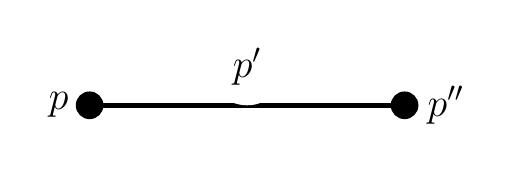
\begin{tikzpicture}[shorten >=1pt, auto, node distance=3cm, ultra thick]
   \begin{scope}[every node/.style={circle,draw=white,fill=white!20!,font=\sffamily\Large\bfseries}]
\coordinate(a) at (0,0);
\coordinate(b) at (4,0);
\draw (a)--(b);
\node [left]  at (a) {$p$};
\node [right]  at (b) {$p^{\prime \prime}$};
\draw  (a) edge node{$p^{\prime}$} (b);
\foreach \p in {a,b}
       \fill [black] (\p) circle (5pt);
  \end{scope}
\end{tikzpicture}
}
\caption{Single link with simultaneous node/link failures. \label{rvrI}}
\end{center}
\end{figure}

\begin{table}[H]
\caption{RVR Validation Test: single link} % title of Table
\centering  % used for centering table
\begin{tabular}{|c|c|c|c|c|} % centered columns 
\hline	$Instance$   &	$R_{s,t}$ & $\hat{R}$&  $\hat{V}$ \\
\hline	$p=p^{\prime}=p^{\prime \prime}=0.9$	& $0.729$ &	$0.729$ 	&	$3.13631E-17$	\\
\hline
\end{tabular}
\label{rvrTable1} % is used to refer this table in the text
\end{table}


\subsubsection*{Case II: Two-Path}
The second test consists of an elementary path composed by two links, with elementary reliability $p^{\prime}$. 
The end-points have reliability $p$, while the central point has reliability $p^{\prime \prime}$ 
(see Figure~\ref{rvrII}). The source-terminal reliability between the end-points is 
$R_{s,t}=p^2(p^{\prime})^2 p^{\prime \prime}$. Table~\ref{rvrTable2} shows a small gap between 
the correct value $R_{s,t}$ and its estimation $\hat{R}$. The estimated variance is reduced as well.

\begin{figure}[H]
\begin{center}
\scalebox{1}{
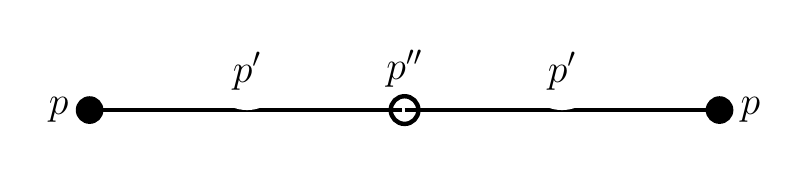
\begin{tikzpicture}[shorten >=1pt, auto, node distance=3cm, ultra thick]
   \begin{scope}[every node/.style={circle,draw=white,fill=white!20!,font=\sffamily\Large\bfseries}]
\coordinate(a) at (0,0);
\coordinate(b) at (4,0);
\coordinate(c) at (8,0);

\draw (a)--(b);
\draw (b)--(c);

\node [left]  at (a) {$p$};
\node [above]  at (b) {$p^{\prime \prime}$};
\node [right]  at (c) {$p$};

\draw  (a) edge node{$p^{\prime}$} (b);
\draw  (b) edge node{$p^{\prime}$} (c);

\foreach \p in {a,c}
       \fill [black] (\p) circle (5pt);
\foreach \p in {b}
       \draw (\p) circle (5pt);
  \end{scope}
\end{tikzpicture}
}      
\caption{Elementary path with simultaneous node/link failures. \label{rvrII}}
\end{center}
\end{figure}

\begin{table}[H]
\caption{RVR Validation Test: elementary path} % title of Table
\centering  % used for centering table
\begin{tabular}{|c|c|c|c|c|} % centered columns 
\hline	$Instance$   &	$R_{s,t}$ & $\hat{R}$&  $\hat{V}$ \\
\hline	$p=p^{\prime}=p^{\prime \prime}=0.9$	& $0.59049$ &	$0.593354$ 	&	$3.3341E-06$	\\
\hline
\end{tabular}
\label{rvrTable2} % is used to refer this table in the text
\end{table}

In the following cases we consider perfect terminals only, with possible failures of Steiner nodes. 
\subsubsection*{Case III: Triangle}
Consider the complete graph composed by three terminal-nodes, or the triangle $K_3$, 
with identical elementary link-reliabilities $p$ (see Figure~\ref{rvrIII}). 
A complete graph with high elementary reliabilities for both links and nodes is therefore highly-reliable. Observe that if two or more links fail, the system is down. 
Otherwise, the system works. By elementary combinatorics, the all-terminal reliability 
is in this case $R_V = \binom{3}{0}p^3+ \binom{3}{1}p^2(1-p) = p^3+3p^2(1-p)$, where the first term means that 
\emph{no link fails}, and the second means that \emph{precisely one link fails}. From Table~\ref{rvrTable3} 
we can observe that the gap between $R_{V}$ and $\hat{R}$ is smaller than $10^{-3}$, and the 
variance is extremely small, showing a good performance of RVR, as expected for small-sized networks. 

\begin{figure}[H]
\begin{center}
\scalebox{1}{
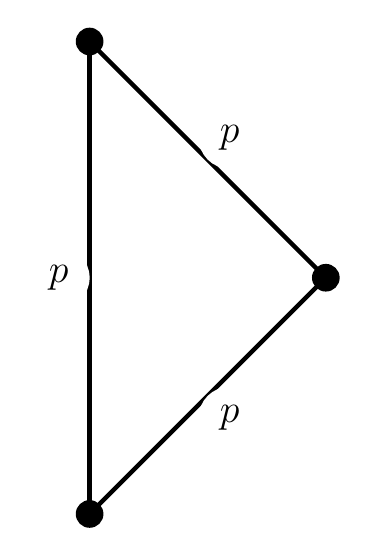
\begin{tikzpicture}[shorten >=1pt, auto, node distance=3cm, ultra thick]
   \begin{scope}[every node/.style={circle,draw=white,fill=white!20!,font=\sffamily\Large\bfseries}]
\coordinate(a) at (0,0);
\coordinate(b) at (0,6);
\coordinate(c) at (3,3);
\draw  (a) edge node{$p$} (b);
\draw  (b) edge node{$p$} (c);
\draw  (c) edge node{$p$} (a);
\foreach \p in {a,b,c}
       \fill [black] (\p) circle (5pt);
  \end{scope}
\end{tikzpicture}
}
\caption{Triangle with link failures. \label{rvrIII}}
\end{center}
\end{figure}

\begin{table}[H]
\caption{RVR Validation Test: Triangle} % title of Table
\centering  % used for centering table
\begin{tabular}{|c|c|c|c|c|} % centered columns 
\hline	$Instance$   &	$R_{V}$ & $\hat{R}$&  $\hat{V}$ \\
\hline	$p=0.9$	& $0.972$ &	$0.972473$ 	&	$6.21454E-08$	\\
\hline
\end{tabular}
\label{rvrTable3} % is used to refer this table in the text
\end{table}

\subsubsection*{Case IV: Triangle with a pending link}
Consider a triangle with a pending link presented in Figure~\ref{rvrIV}, where the central node is a Steiner node (and a cut-point, since it disconnect the network if fails). The $K$-terminal reliability depends strongly on the operational reliabilities of the central node and the bridge. A straight calculation leads to see that 
$R_K = p^{\prime}p^{\prime \prime} [p^3+3p^{2}(1-p)]$. From Table~\ref{rvrTable4}, we can appreciate 
that the gaps in the reliability is again smaller than $10^{-3}$, and the variance of the estimator is really small. 

\begin{figure}[H]
\begin{center}
\scalebox{1}{
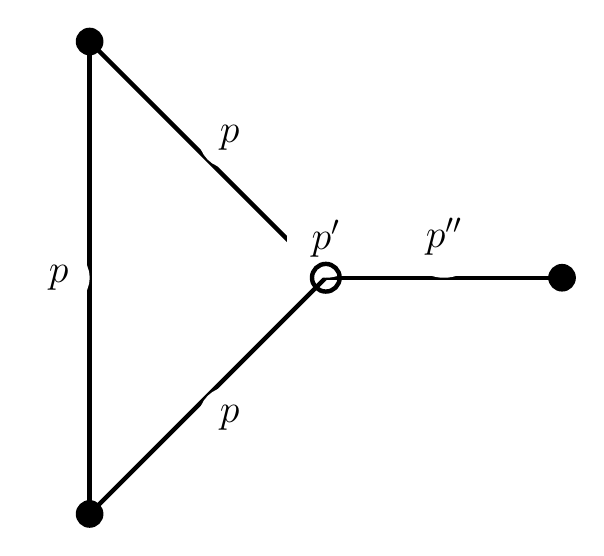
\begin{tikzpicture}[shorten >=1pt, auto, node distance=3cm, ultra thick]
   \begin{scope}[every node/.style={circle,draw=white,fill=white!20!,font=\sffamily\Large\bfseries}]
\coordinate(a) at (0,0);
\coordinate(b) at (0,6);
\coordinate(c) at (3,3);
\coordinate(d) at (6,3);

\draw  (a) edge node{$p$} (b);
\draw  (b) edge node{$p$} (c);
\draw  (c) edge node{$p$} (a);
\draw  (c) edge node{$p^{\prime \prime}$} (d);
\node [above]  at (c) {$p^{\prime}$};

\foreach \p in {a,b,d}
       \fill [black] (\p) circle (5pt);
\foreach \p in {c}
       \draw (\p) circle (5pt);
  \end{scope}
\end{tikzpicture}
}
\caption{Triangle with pending link. Potential failure in central node. \label{rvrIV}}
\end{center}
\end{figure}

\begin{table}[H]
\caption{RVR Validation Test: Triangle with a pending link} % title of Table
\centering  % used for centering table
\begin{tabular}{|c|c|c|c|c|} % centered columns 
\hline	$Instance$   &	$R_{K}$ & $\hat{R}$&  $\hat{V}$ \\
\hline	$p=0.9$, $p^{\prime}=0.5$, $p^{\prime \prime}=0.9$	& $0.4374$ &	$0.438066$ 	&	$3.18052E-07$	\\
\hline	$p=0.9$, $p^{\prime}=0.9$, $p^{\prime \prime}=0.5$		& $0.4374$ &	$0.437479$ 	&	$4.32176E-07$	\\
\hline
\end{tabular}
\label{rvrTable4} % is used to refer this table in the text
\end{table}

\subsubsection*{Case V: Tree}
Consider the tree from Figure~\ref{rvrV}, where the terminals are the leaf-nodes, and all the links and 
Steiner nodes operate independently, with identical reliability. 
In a tree, the failure of only component disconnects some pair of leaf-nodes. Consequently, the reliability 
of trees with several components is reduced, and it is the product of all the elementary reliabilities of its components: $R_K = p^9$. From Table~\ref{rvrTable5}, we can appreciate that both the reliability gap and the variance are greater than in the previous cases. 

\begin{figure}[H]
\begin{center}
\scalebox{1}{
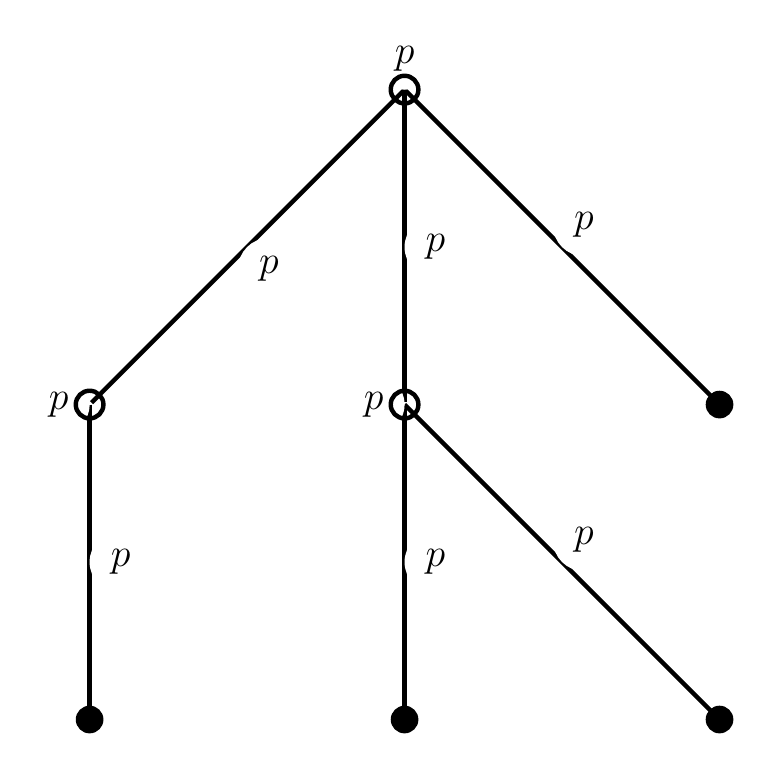
\begin{tikzpicture}[shorten >=1pt, auto, node distance=3cm, ultra thick]
   \begin{scope}[every node/.style={circle,draw=white,fill=white!20!,font=\sffamily\Large\bfseries}]
\coordinate(a) at (0,8);
\coordinate(b) at (4,4);
\coordinate(c) at (0,4);
\coordinate(d) at (-4,4);
\coordinate(e) at (4,0);
\coordinate(f) at (0,0);
\coordinate(g) at (-4,0);

\draw  (a) edge node{$p$} (b);
\draw  (a) edge node{$p$} (c);
\draw  (a) edge node{$p$} (d);
\draw  (c) edge node{$p$} (f);
\draw  (c) edge node{$p$} (e);
\draw  (d) edge node{$p$} (g);

\node [above]  at (a) {$p$};
\node [left]  at (c) {$p$};
\node [left]  at (d) {$p$};

\foreach \p in {b,e,f,g}
       \fill [black] (\p) circle (5pt);
\foreach \p in {a,c,d}
       \draw (\p) circle (5pt);
  \end{scope}
\end{tikzpicture}
}
\caption{Tree with failures in links and non-leaf nodes. \label{rvrV}}
\end{center}
\end{figure}

\begin{table}[H]
\caption{RVR Validation Test: Tree-graph} % title of Table
\centering  % used for centering table
\begin{tabular}{|c|c|c|c|c|} % centered columns 
\hline	$Instance$   &	$R_{K}$ & $\hat{R}$&  $\hat{V}$ \\
\hline	$p=0.9$	& $0.387420489$ &	$0.391676$ 	&	$1.53487e-05$	\\
\hline
\end{tabular}
\label{rvrTable5} % is used to refer this table in the text
\end{table}


\subsubsection*{Case VI: Wheatstone Bridge}
In the Wheatstone Bridge from Figure~\ref{rvrVI}, our measure of interest is the source-terminal reliability 
$R_{s,t}$. It strongly depends on the elementary node-reliability $p^{\prime}$ of Steiner nodes, since these 
represent intermediate nodes. By an exhaustive enumeration of pathsets, a closed-form for the reliability can be obtained:
\begin{equation*}
R_{s,t}= p^2p^{\prime} + p^2(1-p)p^{\prime} + p^3p^{\prime}(1-p^{\prime}) + (1-p)p^3(p^{\prime})^2 + 
p^3(1-p)^2(p^{\prime})^2+ p^3(1-p)^2(p^{\prime})^2.
\end{equation*}

From Table~\ref{rvrTable6}, we conclude that the reliability gaps and variance are acceptable. 
\begin{figure}[H]
\begin{center}
\scalebox{1}{
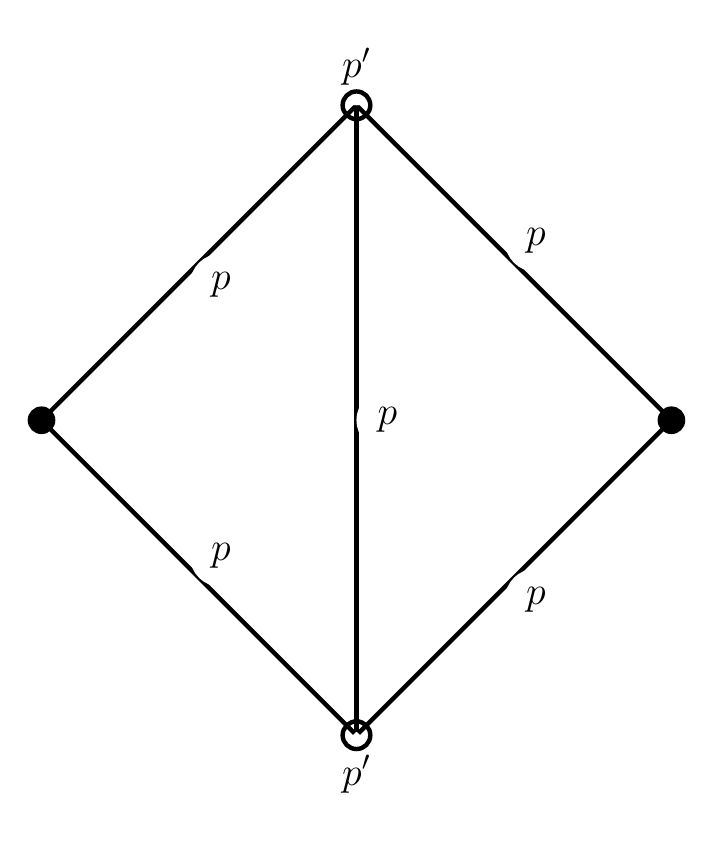
\begin{tikzpicture}[shorten >=1pt, auto, node distance=3cm, ultra thick]
   \begin{scope}[every node/.style={circle,draw=white,fill=white!20!,font=\sffamily\Large\bfseries}]
\coordinate(a) at (0,8);
\coordinate(b) at (4,4);
\coordinate(c) at (-4,4);
\coordinate(d) at (0,0);

\draw  (a) edge node{$p$} (b);
\draw  (a) edge node{$p$} (c);
\draw  (a) edge node{$p$} (d);
\draw  (c) edge node{$p$} (d);
\draw  (b) edge node{$p$} (d);

\node [above]  at (a) {$p^{\prime}$};
\node [below]  at (d) {$p^{\prime}$};


\foreach \p in {b,c}
       \fill [black] (\p) circle (5pt);
\foreach \p in {a,d}
       \draw (\p) circle (5pt);
  \end{scope}
\end{tikzpicture}
}
\caption{Wheatstone Bridge with failures in links and a couple of nodes. \label{rvrVI}}
\end{center}
\end{figure}

\begin{table}[H]
\caption{RVR Validation Test: Wheatstone Bridge} % title of Table
\centering  % used for centering table
\begin{tabular}{|c|c|c|c|c|} % centered columns 
\hline	$Instance$   &	$R_{K}$ & $\hat{R}$&  $\hat{V}$ \\
\hline	$p=0.9$, $p^{\prime}=0.5$	& $0.64962$ &	$0.654653$ 	&	$6.7791E-06$	\\
\hline	$p=0.9$, $p^{\prime}=0.9$	& $0.9383688$ &	$0.937484$ 	&	$1.89235E-06$	\\
\hline
\end{tabular}
\label{rvrTable6} % is used to refer this table in the text
\end{table}

\subsubsection*{Comments on the Results}
Several validation tests were carried out using different elementary reliabilities for nodes and links. 
Some errors were detected during the validation tests, which served to correct the implementation of RVR with 
the corresponding logical modifications. Double-precision arithmetic was used for the operations, with up to 15 digits.